\chapter{Programes per a la calculadora \emph{HP Prime}}\label{sec:progs-HP}
\index{HP Prime}\index{HP Prime!programes}

Es llisten en aquest apèndix una sèrie de programes per a la calculadora \emph{HP Prime} de Hewlett-Packard, els quals són d'interès per resoldre problemes tractats en aquest llibre.

\begin{center}
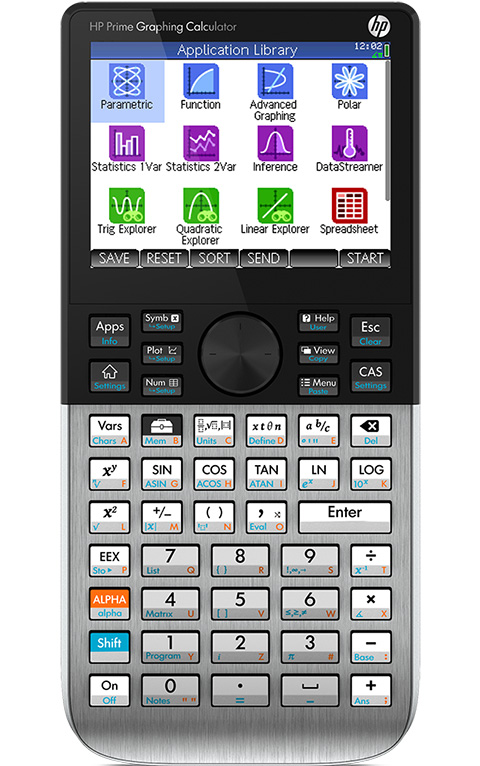
\includegraphics[scale=0.45]{Ape-HP-Prime.jpg}
\end{center}

Aquesta calculadora disposa d'un emulador per a PC, que pot descarregar-se de la pàgina de Hewlett-Packard: \href{http://www.hpprime.de/en/category/6-downloads}{www.hpprime.de/en/category/6-downloads}.

\section{Electrotècnia}\label{sec:HP_ELC}

El programa \funsfbs{Z\_Sèrie} utilitza l'equació \eqref{eq:z_serie} per obtenir la impedància sèrie d'una llista d'impedàncies $\cmplx{Z}_1, \cmplx{Z}_2, ...$; les impedàncies poden ser indistintament reals o complexes.
\vspace{-1cm}
\begin{alltt}
\bfseries
\index{HP Prime!programes!ZSerie@\funsfbs{Z\_Sèrie}}
    EXPORT Z_Sèrie(z)
    // z:impedàncies \{Z1, Z2, ...\} → impedància sèrie
    BEGIN
      RETURN \(\Sigmaup\)LIST(z);
    END;
\end{alltt}

El programa \funsfbs{Z\_Paraŀlel} obté la impedància paraŀlel  d'una llista d'impedàncies $\cmplx{Z}_1, \cmplx{Z}_2, ...$; les impedàncies poden ser indistintament reals o complexes. S'utilitza una variant de l'equació \eqref{eq:z_parallel}, la qual dona una millor precisió numèrica.
\vspace{-1cm}
\begin{alltt}
\bfseries
\index{HP Prime!programes!ZParalel@\funsfbs{Z\_Paraŀlel}}
    EXPORT Z_Paraŀlel(z)
    // z:impedàncies \{Z1, Z2, ...\} → impedància paraŀlel
    BEGIN
      RETURN \(\Piup\)LIST(z)/\(\Sigmaup\)LIST(\(\Piup\)LIST(z)/z);
    END;
\end{alltt}

El programa \funsfbs{Millman} utilitza l'equació \eqref{eq:millman} per obtenir la tensió $\cmplx{U}\ped{nx}$ del punt neutre $n$ d'una llista d'impedàncies connectades en estrella $\cmplx{Z}\ped{an}, \cmplx{Z}\ped{bn}, \cmplx{Z}\ped{cn}, ...$, respecte d'un punt qualsevol $x$, a partir de la llista de tensions $\cmplx{U}\ped{ax}, \cmplx{U}\ped{bx}, \cmplx{U}\ped{cx}, ...$ dels extrems d'aquestes impedàncies respecte del mateix punt $x$; les impedàncies i les tensions poden ser indistintament reals o complexes. És necessari el programa \funsfbs{Z\_Paraŀlel}, definit anteriorment.
\vspace{-1cm}
\begin{alltt}
\bfseries
\index{HP Prime!programes!Millman@\funsfbs{Millman}}
    EXPORT Millman(u,z)
    // u:tensions \{Uax,Ubx,Ucx,...\}, z:impedàncies \{Zan,Zbn,Zcn,...\} → tensió Unx
    // n és el punt neutre de les impedàncies, i x és un punt qualsevol
    BEGIN
      RETURN \(\Sigmaup\)LIST(u ./ z) * Z_Paraŀlel(z);
    END;
\end{alltt}


El programa \funsfbs{Triangle\_a\_Estrella} utilitza l'equació \eqref{eq:Y_D} per transformar una llista de tres impedàncies connectades en triangle $\cmplx{Z}\ped{ab}$, $\cmplx{Z}\ped{bc}$ i  $\cmplx{Z}\ped{ca}$, en una llista de tres impedàncies equivalents connectades en estrella $\cmplx{Z}\ped{an}$, $\cmplx{Z}\ped{bn}$ i $\cmplx{Z}\ped{cn}$; les impedàncies poden ser indistintament reals o complexes.
\vspace{-1cm}
\begin{alltt}
\bfseries
\index{HP Prime!programes!TriangleaEstrella@\funsfbs{Triangle\_a\_Estrella}}
    EXPORT Triangle_a_Estrella(zd)
    // zd:impedàncies en triangle \{Zab,Zbc,Zca\} → impedàncies en
    // estrella \{Zan,Zbn,Zcn\}
    BEGIN
      LOCAL z:=\(\Piup\)LIST(zd)/\(\Sigmaup\)LIST(zd);
      RETURN \{z/zd(2),z/zd(3),z/zd(1)\};
    END;
\end{alltt}

El programa \funsfbs{Estrella\_a\_Triangle} utilitza l'equació \eqref{eq:Y_D} per transformar una llista de tres impedàncies connectades en estrella $\cmplx{Z}\ped{an}$, $\cmplx{Z}\ped{bn}$ i $\cmplx{Z}\ped{cn}$, en una llista de tres impedàncies equivalents connectades en triangle $\cmplx{Z}\ped{ab}$, $\cmplx{Z}\ped{bc}$ i  $\cmplx{Z}\ped{ca}$; les impedàncies poden ser indistintament reals o complexes.
\vspace{-1cm}
\begin{alltt}
\bfseries
\index{HP Prime!programes!EstrellaaTriangle@\funsfbs{Estrella\_a\_Triangle}}
    EXPORT Estrella_a_Triangle(zy)
    // zy:impedàncies en estrella \{Zan,Zbn,Zcn\} → impedàncies en
    // triangle \{Zab,Zbc,Zca\}
    BEGIN
      LOCAL z:=zy(1)*(zy(2)+zy(3))+zy(2)*zy(3);
      RETURN \{z/zy(3),z/zy(1),z/zy(2)\};
    END;
\end{alltt}

El programa \funsfbs{EZS\_U} utilitza les equacions de la secció \vref{sec:EZS} per obtenir la tensió $\cmplx{U}$ d'una carrega que absorbeix una potència $\cmplx{S}$, quan està connectada a una font de tensió $\cmplx{E}$ a través d'una impedància $\cmplx{Z}$; cadascun d'aquests valors pot ser indistintament real o complex.
\vspace{-1cm}
\begin{alltt}
\bfseries
\index{HP Prime!programes!EZSU@\funsfbs{EZS\_U}}
    EXPORT EZS_U(E,Z,S)
    // E:font de tensió, Z:impedància, S:potència de la càrrega → tensió U
    // de la càrrega
    BEGIN
      LOCAL ZcS:=CONJ(Z)*S;
      LOCAL ImUe:=IM(ZcS)/ABS(E);
      LOCAL ReUe:=POLYROOT(\{1,-ABS(E),RE(ZcS)+ImUe^2\});
      IF TYPE(ReUe(1))==3 THEN
        RETURN "No hi ha solució"; // Arrels complexes
      ELSE
        RETURN (MAX(ReUe),ImUe)*SIGN(E);
      END;
    END;
\end{alltt}


El programa \funsfbs{kcmil\_a\_mm2} utilitza l'equació \eqref{eq:kcmil_mm2} per convertir la secció d'un conductor expressada en \si{kcmil}, en la seva secció equivalent expressada en \si{mm^2}.
\vspace{-1cm}
\begin{alltt}
\bfseries
\index{HP Prime!programes!kcmilamm2@\funsfbs{kcmil\_a\_mm2}}
    EXPORT kcmil_a_mm2(kcmil)
    // kcmil:secció en kcmil → secció en mm²
    BEGIN
      RETURN kcmil*0.506707479098;
    END;
\end{alltt}

El programa \funsfbs{mm2\_a\_kcmil} utilitza l'equació \eqref{eq:kcmil_mm2} per convertir la secció d'un conductor expressada en \si{mm^2}, en la seva secció equivalent expressada en \si{kcmil}.
\vspace{-1cm}
\begin{alltt}
\bfseries
\index{HP Prime!programes!mm2akcmil@\funsfbs{mm2\_a\_kcmil}}
    EXPORT mm2_a_kcmil(mm2)
    // mm2:secció en mm² → secció en kcmil
    BEGIN
      RETURN mm2/0.506707479098;
    END;
\end{alltt}

El programa \funsfbs{AWG\_a\_mm2} utilitza l'equació \eqref{eq:awg_mm2} per convertir la secció d'un conductor expressada segons el seu número AWG, en la seva secció equivalent expressada en \si{mm^2}.
\vspace{-1cm}
\begin{alltt}
\bfseries
\index{HP Prime!programes!AWGamm2@\funsfbs{AWG\_a\_mm2}}
    EXPORT AWG_a_mm2(AWG)
    // AWG:número AWG → secció en mm²
    // cal entrar 0, -1, -2 i -3 en el cas dels números AWG 1/0, 2/0, 3/0 i 4/0
    BEGIN
      RETURN 53.4751207321/(92^(AWG/19.5));
    END;
\end{alltt}

El programa \funsfbs{mm2\_a\_AWG} utilitza l'equació \eqref{eq:mm2_awg} per convertir la secció d'un conductor expressada en \si{mm^2}, en la seva secció equivalent expressada segons el seu número AWG; la conversió és aproximada ja que els números AWG prenen valors discrets.
\vspace{-1cm}
\begin{alltt}
\bfseries
\index{HP Prime!programes!mm2aAWG@\funsfbs{mm2\_a\_AWG}}
    EXPORT mm2_a_AWG(mm2)
    // mm2:secció en mm² → número AWG més proper
    // els resultats 0, -1, -2 i -3 són equivalents als números
    // AWG 1/0, 2/0, 3/0 i 4/0
    BEGIN
      RETURN ROUND(4.31245284200*LN(53.4751207321/mm2),0);
    END;
\end{alltt}


El programa \funsfbs{Triangle\_a\_Fasors} obté els tres fasors $\cmplx{U}\ped{AB}$, $\cmplx{U}\ped{BC}$ i $\cmplx{U}\ped{CA}$ que formen un triangle de tensions fase--fase, a partir de les longituds dels tres costats d'aquest triangle $|\cmplx{U}\ped{AB}|$, $|\cmplx{U}\ped{BC}|$ i $|\cmplx{U}\ped{CA}|$. Es pren $\cmplx{U}\ped{AB}$ com a fasor de referència.
\vspace{-1cm}
\begin{alltt}
\bfseries
\index{HP Prime!programes!TriangleaFasors@\funsfbs{Triangle\_a\_Fasors}}
    EXPORT Triangle_a_Fasors(u)
    // u:triangle de tensions \{Uab,Ubc,Uca\} → fasors de tensió \{Uab,Ubc,Uca\}
    // la tensió Uab es pren com el fasor de referència (angle igual a zero)
    BEGIN
      LOCAL \(\varphiup\):=Triangle_Solver.SSS(u(1),u(3),u(2));
      RETURN \{u(1),u(2)*(-1,0)*(1,\(\measuredangle\varphiup\)(2)),u(3)*(-1,0)/(1,\(\measuredangle\varphiup\)(3))\};
    END;
\end{alltt}

El programa \funsfbs{FN\_a\_FF} obté els fasors de les tres tensions fase--fase $\cmplx{U}\ped{AB}$, $\cmplx{U}\ped{BC}$ i $\cmplx{U}\ped{CA}$, corresponents als fasors de les tres tensions fase--neutre
$\cmplx{U}\ped{AN}$, $\cmplx{U}\ped{BN}$ i $\cmplx{U}\ped{CN}$.
\vspace{-1cm}
\begin{alltt}
\bfseries
\index{HP Prime!programes!FNaFF@\funsfbs{FN\_a\_FF}}
    EXPORT FN_a_FF(u)
    // u:tensions fase-neutre \{Uan,Ubn,Ucn\} → tensions fase-fase \{Uab,Ubc,Uca\}
    BEGIN
      RETURN \{u(1)-u(2),u(2)-u(3),u(3)-u(1)\};
    END;
\end{alltt}

El programa \funsfbs{FF\_a\_FN} obté els fasors de les tres tensions fase--neutre $\cmplx{U}\ped{AN}$, $\cmplx{U}\ped{BN}$ i $\cmplx{U}\ped{CN}$, corresponents a tres impedàncies $\cmplx{Z}\ped{AN}$, $\cmplx{Z}\ped{BN}$ i $\cmplx{Z}\ped{CN}$ connectades en estrella a  les tres tensions fase--fase
$\cmplx{U}\ped{AB}$, $\cmplx{U}\ped{BC}$ i $\cmplx{U}\ped{CA}$.
\pagebreak
\begin{alltt}
\bfseries
\index{HP Prime!programes!FFaFN@\funsfbs{FF\_a\_FN}}
    EXPORT FF_a_FN(u,z)
    // u:tensions fase-fase \{Uab,Ubc,Uca\}, z:impedàncies \{Zan,Zbn,Zcn\} →
    // tensions fase-neutre \{Uan,Ubn,Ucn\}
    BEGIN
      RETURN \{u(1)/z(2)-u(3)/z(3),u(2)/z(3)-u(1)/z(1),
              u(3)/z(1)-u(2)/z(2)\}*Z_Paraŀlel(z);
    END;
\end{alltt}

El programa \funsfbs{FF\_a\_FG} obté els fasors de les tres tensions fase--neutre $\cmplx{U}\ped{AG}$, $\cmplx{U}\ped{BG}$ i $\cmplx{U}\ped{CG}$ que tenen el punt neutre G en el baricentre del triangle format pels fasors de  les tres tensions fase--fase
$\cmplx{U}\ped{AB}$, $\cmplx{U}\ped{BC}$ i $\cmplx{U}\ped{CA}$. És un cas particular del programa anterior, quan les tres impedàncies són idèntiques.
\vspace{-1cm}
\begin{alltt}
\bfseries
\index{HP Prime!programes!FFaFG@\funsfbs{FF\_a\_FG}}
    EXPORT FF_a_FG(u)
    // u:tensions fase-fase \{Uab,Ubc,Uca\} → tensions fase-G \{Uag,Ubg,Ucg\}
    // G is el baricentre del triangle de tensions fase-fase
    BEGIN
      RETURN \{u(1)-u(3),u(2)-u(1),u(3)-u(2)\}/3;
    END;
\end{alltt}

El programa \funsfbs{ABC\_a\_A012} utilitza l'equació \eqref{eq:c_sim_mat1} per obtenir els tres fasors de seqüència
$\cmplx{A}_0$, $\cmplx{A}_1$ i  $\cmplx{A}_2$ corresponents als tres fasors $\cmplx{A}$, $\cmplx{B}$ i $\cmplx{C}$.
\vspace{-1cm}
\begin{alltt}
\bfseries
\index{HP Prime!programes!ABCaA012@\funsfbs{ABC\_a\_A012}}
    EXPORT ABC_a_A012(x)
    // x:fasors \{A,B,C\} → fasors de seqüència \{A0,A1,A2\}
    BEGIN
      LOCAL A:=[[1,1,1],[1,(-1/2,\(\sqrt{\phantom{|}}\)3/2),(-1/2,-\(\sqrt{\phantom{|}}\)3/2)],
                [1,(-1/2,-\(\sqrt{\phantom{|}}\)3/2),(-1/2,\(\sqrt{\phantom{|}}\)3/2)]];
      RETURN mat2list(A*list2mat(x,1)/3);
    END;
\end{alltt}

El programa \funsfbs{A012\_a\_ABC} fa la funció inversa del programa anterior, i utilitza l'equació \eqref{eq:c_sim_mat} per obtenir els tres fasors
$\cmplx{A}$, $\cmplx{B}$ i $\cmplx{C}$  corresponents als tres fasors de seqüència
$\cmplx{A}_0$, $\cmplx{A}_1$ i  $\cmplx{A}_2$.
\vspace{-1cm}
\begin{alltt}
\bfseries
\index{HP Prime!programes!A012aABC@\funsfbs{A012\_a\_ABC}}
    EXPORT A012_a_ABC(x)
    // x:fasors de seqüència \{A0,A1,A2\} → fasors \{A,B,C\}
    BEGIN
      LOCAL A:=[[1,1,1],[1,(-1/2,-\(\sqrt{\phantom{|}}\)3/2),(-1/2,\(\sqrt{\phantom{|}}\)3/2)],
                [1,(-1/2,\(\sqrt{\phantom{|}}\)3/2),(-1/2,-\(\sqrt{\phantom{|}}\)3/2)]];
      RETURN mat2list(A*list2mat(x,1));
    END;
\end{alltt}

El programa \funsfbs{AN12\_a\_AB12} utilitza les equacions  \eqref{eq:c_sim_a3} i \eqref{eq:c_sim_b3} per obtenir els dos fasors de tensions de seqüència fase--fase $\cmplx{U}\ped{AB,1}$ i  $\cmplx{U}\ped{AB,2}$ a partir dels dos fasors de tensions de seqüència fase--neutre $\cmplx{U}\ped{AN,1}$ i $\cmplx{U}\ped{AN,2}$.
\pagebreak
\begin{alltt}
\bfseries
\index{HP Prime!programes!AN12aAB12@\funsfbs{AN12\_a\_AB12}}
    EXPORT AN12_a_AB12(x)
    // x:fasors de seqüència fase-neutre \{AN1,AN2\} → fasors de seqüència
    // fase-fase \{AB1,AB2\}
    BEGIN
      RETURN \(\sqrt{\phantom{|}}\)3*\{x(1)*exp(\(\piup\)*i/6),x(2)*exp(-\(\piup\)*i/6)\};
    END;
\end{alltt}

El programa \funsfbs{AB12\_a\_AN12} fa la funció inversa del programa anterior, i utilitza les mateixes equacions  \eqref{eq:c_sim_a3} i \eqref{eq:c_sim_b3} per obtenir els dos fasors de tensions de seqüència fase--neutre $\cmplx{U}\ped{AN,1}$ i $\cmplx{U}\ped{AN,2}$ a partir dels dos fasors de tensions de seqüència fase--fase $\cmplx{U}\ped{AB,1}$ i  $\cmplx{U}\ped{AB,2}$:
\vspace{-1cm}
\begin{alltt}
\bfseries
\index{HP Prime!programes!AB12aAN12@\funsfbs{AB12\_a\_AN12}}
    EXPORT AB12_a_AN12(x)
    // x:fasors de seqüència fase-fase \{AB1,AB2\} → fasors de seqüència
    // fase-neutre {AN1,AN2}
    BEGIN
      RETURN \{x(1)/exp(\(\piup\)*i/6),x(2)/exp(-\(\piup\)*i/6)\}/\(\sqrt{\phantom{|}}\)3;
    END;
\end{alltt}


\section{Matemàtiques}

El programa \funsfbs{Interpolació\_Polinòmica} obté la ordenada interpolada $y$ corresponent a una abscissa $x$, a partir d'un conjunt  de punts $(x_1,y_1)$, $(x_2,y_2)$, ..., $(x\ped{n},y\ped{n})$. S'utilitza una interpolació polinòmica, obtenint el mateixos resultats que amb el mètode descrit en la secció \vref{sec:poli_lagr}; el grau del polinomi és igual a $n-1$.
\vspace{-1cm}
\begin{alltt}
\bfseries
\index{HP Prime!programes!InterpolacióPolinòmica@\funsfbs{Interpolació\_Polinòmica}}
    EXPORT Interpolació_Polinòmica(dades,x)
    // dades:[[x1,y1], x:abscissa → ordenada y interpolada
    //        [x2,y2]
    //        .......
    //        [xn,yn]]
    BEGIN
      RETURN POLYEVAL(polynomial_regression(dades,rowDim(dades)-1),x);
    END;
\end{alltt}


El programa \funsfbs{Interpolació\_Polinòmica\_2dim} obté el valor interpolat $z$ corresponent a un punt $(x, y)$, a partir d'un conjunt de punts $(x\ped{1}, x\ped{2}, ... x\ped{n})$, d'un conjunt de punts $(y\ped{1}, y\ped{2}, ... y\ped{m})$, i d'una matriu de valors $(z\ped{11}, z\ped{12}, ..., z\ped{1n})$,
$(z\ped{21}, z\ped{22}, ..., z\ped{2n})$, ..., $(z\ped{m1}, z\ped{m2}, ..., z\ped{mn})$. S'utilitzen  interpolacions polinòmiques, obtenint el mateixos resultats que amb el mètode descrit en la secció \vref{sec:poli_lagr}; el grau dels polinomis és igual a $n-1$ i $m-1$.
És necessari el programa \funsfbs{Interpolació\_Polinòmica}, definit anteriorment.
\vspace{-1cm}
\begin{alltt}
\bfseries
\index{HP Prime!programes!InterpolacióPolinòmica2dim@\funsfbs{Interpolació\_Polinòmica\_2dim}}
    EXPORT Interpolació_Polinòmica_2dim(dades,x,y)
    // dades:[[0,   x1,  x2, ...  xn], x, y → z interpolada
    //        [y1, z11, z12, ... z1n]
    //        [y2, z21, z22, ... z2n]
    //        .......................
    //        [ym, zm1, zm2, ... zmn]]
    BEGIN
      LOCAL c:=colDim(dades);
      LOCAL r:=rowDim(dades);
      LOCAL d:=[[0,0],[0,0]];
      LOCAL z:=[[0,0],[0,0]];
      LOCAL k;
      d(-1):=dades(\{\{1,2\},\{1,c\}\});
      FOR k FROM 2 TO r DO
        d(-2):=dades(\{\{k,2\},\{k,c\}\});
        z(k-1,2):=Interpolació_Polinòmica(d,x);
      END;
      z(-1):=TRN(dades(\{\{2,1\},\{r,1\}\}));
      RETURN Interpolació_Polinòmica(z,y);
    END;
\end{alltt}

El programa \funsfbs{Regla\_dels\_Trapezis} utilitza l'equació  \eqref{eq:trap-uneven} per obtenir la integral entre $x_1$ i $x_n$ d'un conjunt  de punts $(x_1,y_1)$, $(x_2,y_2)$, ..., $(x\ped{n},y\ped{n})$, utilitzant la regla dels trapezis.
\vspace{-1cm}
\begin{alltt}
\bfseries
\index{HP Prime!programes!RegladelsTrapezis@\funsfbs{Regla\_dels\_Trapezis}}
    EXPORT Regla_dels_Trapezis(dades)
    // dades:[[x1,y1] → Integral de x1 a xn
    //        [x2,y2]
    //        .......
    //        [xn,yn]]
    BEGIN
      LOCAL k;
      LOCAL a:=0;
      LOCAL n:=rowDim(dades)-1;
      FOR k FROM 1 TO n DO
        a:=a+(dades(k+1,2)+dades(k,2))*(dades(k+1,1)-dades(k,1));
      END;
      RETURN a/2;
    END;
\end{alltt}
